% for two sided printing
%\documentclass[11pt,a4paper,twoside]{book}
% for one sided printing
\documentclass[11pt,a4paper,oneside]{book}
% A few packages that you might need - I have included all the ones that are needed for this template to work correctly, plus a few more. If you wish to do more with Latex then you may need to import other ones. 
\usepackage{amsmath,amssymb,amsthm,color,enumerate,graphicx,stackrel,natbib,setspace,ifthen,url,array,theorem,pifont}
\usepackage{lscape}
\usepackage{placeins}
\usepackage{multirow}
\usepackage{fancyhdr}
\usepackage{emptypage}
% For printing with binding
\usepackage[inner=4cm,outer=2cm,top=2.5cm,bottom=3cm]{geometry}
% For pdf or printing without binding
% \usepackage[inner=3cm,outer=3cm,top=2.5cm,bottom=3cm]{geometry}
\usepackage[sc]{titlesec}

%\usepackage[toc,page]{appendix}
\usepackage[titletoc,title]{appendix}
%\input{FloatSettings} % For things like figures and tables
%\input{BibSettings}   % For bibliographies
\linespread{1.3}
% Title Settings
\setcounter{secnumdepth}{3}
\setcounter{tocdepth}{3}
\usepackage{hyperref}
\usepackage{doi}
\begin{document}
\pagestyle{plain}
\frontmatter
%Create a title page
\begin{titlepage} % Suppresses displaying the page number on the title page and the subsequent page counts as page 1
	\newcommand{\HRule}{\rule{\linewidth}{0.5mm}} % Defines a new command for horizontal lines, change thickness here
	
	\center % Centre everything on the page
	%------------------------------------------------
	%	Headings
	%------------------------------------------------	
	\textsc{\LARGE University College London}\\[1.5cm] % Main heading institution
	
	\textsc{\Large Department of Computer Science}\\[0.5cm] % Major heading department
	
	\textsc{\large A thesis submitted in partial fulfilment of the requirements for the degree of Master of Science in Computational Finance/Financial Risk Management, University College London}\\[0.5cm] % Minor heading such as course title	
	%------------------------------------------------
	%	Title
	%------------------------------------------------
	\HRule\\[0.4cm]
	\textsc{\huge Dissertation title}\\[0.4cm] % Title of your document
	\HRule\\[1.5cm]
	%------------------------------------------------
	%	Author and Supervisor
	%------------------------------------------------
	{\large\textit{Author}}\\
	Firstname \textsc{Surname} % Your name
	\vfill
	\begin{minipage}{0.48\textwidth}
		\begin{flushleft}
			\large
			\textit{Academic Supervisor}\\
			Title (e.g.~Mr/Ms/Dr) Firstname \textsc{Second name}\\ % Supervisor's name
			\textsc{Department of Computer Science}\\
			\textsc{University College London}
		\end{flushleft}
	\end{minipage}
	~% Fill in the next one for your industrial supervisor - if you do not have one put your second marker
	\begin{minipage}{0.48\textwidth}
		\begin{flushright}
			\large
			\textit{Industrial Supervisor}\\
			Title (e.g.~Mr/Ms/Dr) Firstname  \textsc{Second name}\\ % Supervisor's name
			\textsc{Department}\\%Department
			\textsc{Company name}%Company name
		\end{flushright}
	\end{minipage}
	%------------------------------------------------
	%	Date
	%------------------------------------------------	
	\vfill\vfill\vfill % Position the date 3/4 down the remaining page	
	
	{\large\textit\today} % Date, change the \today to a set date if you want to be precise
	
	%------------------------------------------------
	%	Logo
	%------------------------------------------------
       \includegraphics[width=0.2\textwidth]{ucl_logo}\\[1cm] % Include a department/university logo - this will require the graphicx package
	%------------------------------------------------
	%	Disclaimer
	%------------------------------------------------
	
	% Uncomment one of the following statements as appropriate.
	
	 This dissertation is submitted as part requirement for the MSc ... degree at UCL. It is substantially the result of my own work except where explicitly 	indicated in the text. 
	 
	 %The dissertation may be freely copied and distributed provided the source is explicitly acknowledged.

	%Or if your project includes information that prevents it from being more widely circulated:
	
	% This dissertation is submitted as part requirement for the MSc ? degree at UCL. It is substantially the result of my own work except where explicitly 	indicated in the text. The dissertation will be distributed to the internal and external examiners, but thereafter may not be copied or distributed except 	with permission from the author.

	%\vfill % Push the date up 1/4 of the remaining page
	
\end{titlepage}
\clearpage 
\newpage 

%\mbox{} % comment this line out for single sided printing
%\newpage % comment this line out for single sided printing
 
% If you wish to dedication your thesis to anyone then you can add this by uncommenting out the following 11 lines
%\section*{Dedications}
%\vspace*{20mm}
%\begin{center}
%\begin{minipage}{0.8\textwidth}
%Dedication
%\end{minipage}
%\end{center}
%\newpage
%\mbox{} % comment this line out for single sided printing
%\newpage % comment this line out for single sided printing

\section*{Abstract}
This \LaTeX\ template is intended to to help you in your writing by providing a framework for your MSc dissertation. It is not intended to be prescriptive and you are welcome to change it or use a different one as long as it contains all the required elements
\newpage 
%\mbox{} % comment this out for single sided printing
%\newpage % comment this out for single sided printing
\section*{Acknowledgments}
Write any acknowledgments that you wish to include here e.g.~supervisors/family/etc. You should also include a mention of any grants, sponsorship or other funding that you have received to help you undertake your MSc course.
\newpage
% The table of contents, list of figures and list of tables go here
\setcounter{tocdepth}{2} 
% Setting this higher means you get contents entries for
%  more minor section headers.
\cleardoublepage
\tableofcontents
\cleardoublepage
\listoffigures
\cleardoublepage
\listoftables

% Start the main part of the document here.
\mainmatter
\chapter{Chapter title}
\section{Section title}\label{sec:1_example1}
This \LaTeX\ template is intended to to help you in your writing by providing a framework for your MSc dissertation. It is not intended to be prescriptive and you are welcome to change it or use a different one. Furthermore, your academic supervisor may have their own preferences with regards to the layout and format of your dissertation, in which case you should follow their direction. In any event, your dissertation should have a neat and professional appearance and include the following elements in addition to the core content:
\begin{enumerate}
\item Title
\item Student name
\item Academic supervisor name
\item Industrial supervisor name (if applicable)
\item Disclaimer
\item Table of contents
\item List of figures
\item List of tables
\item Bibliography
\end{enumerate}
In this template I have included a few examples of \LaTeX\ commands, but for more details there are numerous resources online. For those of you who prefer print, a useful book is \cite{Lamport1994}.

\subsection{Subsection title}
\subsubsection{Subsubsection title}
Example of a figure:
%If you wish to create a figure then use something like 
\begin{figure}[h]
\begin{center}
\includegraphics[width=0.48\textwidth]{subfig1.eps}\hfill
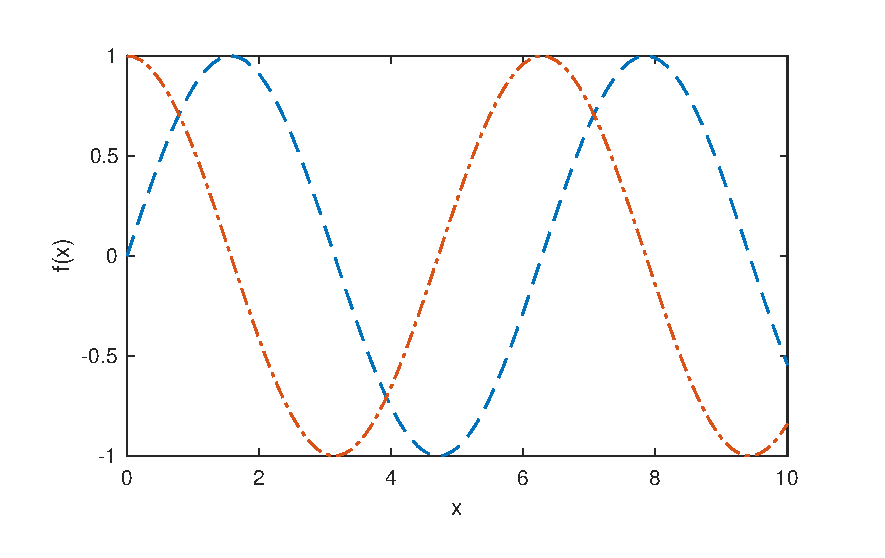
\includegraphics[width=0.48\textwidth]{subfig2.eps}
\caption[Short figure title]{It is good practice to put a long descriptive title in your caption so that readers can immediately understand the significance of the figure without having to search through the accompanying text. The short title in square brackets before the long caption is for the more concise description included in the List of figures.}
\label{fig:1_example1}
\end{center}
\end{figure}
\FloatBarrier The use of ``\textbackslash FloatBarrier'' allows you to specify that floats (e.g. Figures and Tables) should not appear past a certain point in a document but you must import the ``placeins'' package in order to use it.


Example of a table:
% If you wish to include a table then use something like
\begin{table}[ht]
\begin{center}
\begin{tabular}{lllr}
\hline\hline
\multicolumn{4}{c}{Process parameters}\\
\hline
Process & $\Psi(\xi,t)$ & Symbol & Value\\
\hline
\multirow{2}{*}{Gaussian}&\multirow{2}{*}{$e^{\big(i\mu\xi-\frac{1}{2}\sigma^2\xi^2\big)t}$} & $\mu$ & 0\\
& & $\sigma$ & 0.4\\
\hline
\multirow{3}{*}{Variance gamma}&\multirow{3}{*}{$\big(1-i\nu\xi\theta+\frac{1}{2}\nu\sigma^2\xi^2\big)^{-\frac{t}{\nu}}$} & $\theta$ & $\frac{1}{9}$\\
\noalign{\vskip 0.5mm}
& & $\sigma$ &$\frac{1}{3\sqrt{3}}$\\
\noalign{\vskip 0.5mm}
& & $\nu$ & 0.25 \\
\hline
\multirow{4}{*}{Merton jump-diffusion}&\multirow{4}{*}{$e^{\big(-\frac{1}{2}\sigma^2\xi^2+\lambda(e^{i\mu_\mathrm{J}\xi-\frac{1}{2}\sigma_\mathrm{J}^2\xi^2}-1)\big)t}$} & $\sigma$ & 0.1\\
\noalign{\vskip 0.5mm}
& & $\lambda$ &3\\
\noalign{\vskip 0.5mm}
& & $\mu_J$ & -0.05 \\
\noalign{\vskip 0.5mm}
& & $\sigma_J$ & 0.086\\
\hline\hline
\end{tabular}
\end{center}
\caption[Example table using multirow and multicolumn]{This is an example table, you end a column entry using \& and a row entry with the usual double backslash. Notice that you can use in text formulas surrounded by the usual \$\$. You can also merge columns and rows using the multicolumn and multirow commands but you must import the multirow package to do this.}
\label{tab:1_example1}
\end{table}

In order to include formulas, you can use in line equations by using \$ at the beginning and end, for example $y=f(x)$ and single line equations using the ``equation'' environment, for example
\begin{equation}
f(x)=\frac{1}{2\pi}\int^{+\infty}_{-\infty}e^{-ix\xi}\widehat{f}(\xi)d\xi.
\end{equation}
You can also write equations on several lines using the ``align'' environment, notice the use of \& at the point where the lines align and the double backslash to move to the next line, for example
\begin{align}
f(x)&=\frac{1}{2\pi}\int^{+\infty}_{-\infty}e^{-ix\xi}\widehat{f}(\xi)d\xi \nonumber\\
&=\frac{1}{2\pi}\int^{+\infty}_{-\infty}e^{-ix\eta}\widehat{f}(\eta)d\eta. \label{eq:1_example1}
\end{align}
Notice the use of ``\textbackslash nonumber'' above to suppress the equation numbering on the first line.

You can also use the ``\textbackslash label\{\}'' ``\textbackslash ref\{\}'' commands to reference items in the dissertation such as Section \ref{sec:1_example1}, Figure \ref{fig:1_example1}, Table \ref{tab:1_example1} and Eq.~(\ref{eq:1_example1}).

You must also include a bibliography so that you can reference your background reading. This should include papers, for example \cite{fusai2015}, books, for example \cite{Press2007}, and websites, for example \cite{Wang2014}.

Write your bibliography as a .bib file (an example is included) and then import using the ``\textbackslash bibliography\{\}'' command.

\addcontentsline{toc}{chapter}{Bibliography} % adds a page number for the bibliography to the table of contents

% Actually generates your bibliography.
\bibliographystyle{ormsv080}
\bibliography{MSc_template_tex_examplebib}

% You can use the appendices to include additional items, such as code listings, which are not vital to understand your work but may be of interest to the reader.
\begin{appendices}
\chapter{Title of first appendix}
\section{Code listing}
If you wish to list code in your appendices, one way is to use the ``verbatim" environment.

\begin{verbatim}
% Left hand side plot
figure
plot(1:10,(1:10).^2,'--',1:10,((1:10).^2)/2,'-.','Linewidth',1)
xlabel('x')
ylabel('f(x)')
% Right hand side plot
figure
plot(0:0.1:10,sin(0:0.1:10),'--',0:0.1:10,cos(0:0.1:10),'-.','Linewidth',1)
xlabel('x')
ylabel('f(x)')
\end{verbatim}

\end{appendices}
\end{document}